\documentclass[11pt]{article}
\usepackage{float}
\usepackage{acl2014}
\usepackage{times}
\usepackage{url}
\usepackage{subfig}
\usepackage{graphicx}
\usepackage{latexsym}
\usepackage{breqn}

%\setlength\titlebox{5cm}

\title{On data selection for statistical machine translation.}
\author{Anouk Visser \& R\'emi de Zoeten}
\date{}

\begin{document}

\maketitle

\begin{abstract}
HY
\end{abstract}

\section{Introduction}
\label{sec:intro}
The performance of a Statistical Machine Translation (SMT) systems is dependent on the data that is used to train the model. For accurate translations it is useful to base the model on training data that matches the domain where the machine translation will be applied. When translating a text about software, ideally, the sentences in the training corpus should be cherry picked from a software domain. 
In this work we investigate how to extract in-domain sentences from a large mixed-domain training corpus. We develop and evaluate several methods to order a set of training sentences based on the estimated likelihood that the sentence pair is in-domain. The top-$n$ sentences are then used for training a translation system and comparing the performance to a system that is trained with $n$ sentence pairs that were randomly selected from the mixed-domain corpus.
%The paper is organized as follows. Section \ref{sec:related} describes related work, section \ref{sec:methods} explains the different methods that we have used for sentence-reordering, section \ref{sec:results} shows the performance of our methods in terms of sentence-reordering ability and the effects this has on translation performance, and finally we end with some concluding remarks \ref{sec:conclusion}.

\section{Experimental Setting}
Our data consists of three parallel corpora (English-Spanish). There are $100.000$ sentence pairs in the software domain, $100.000$ in the legal domain and $450.000$ in the general domain corpus. 

We have split these three corpora in a training and a test set. The training data consists of $50.000$ sentence pairs for the software domain and the legal domain, as well as $50.000$ sentence pairs from the general domain dataset.

Our test data consists of a general domain dataset of $400.000$ sentences, which is combined with $50.000$ in-domain sentences to create two sets of $450.000$ sentence pairs that need to be ranked according to their relevance to the domain.

\subsection{Pseudo Recall}
In addition to selecting data that is relevant to a specific domain, we are interested in ranking the selected data according to its relevance to the domain. To evaluate our data selection performance we create a set of $450.000$ sentences of which we know which $50.000$ sentences belong to the domain. Ideally, when asked to select $50.000$ sentences, our system would select all in-domain sentences resulting in a $\textit{recall@}50.000$ of $1$. We compute \textit{recall@k} as: 
$$ \textit{recall@k} = \frac{\textit{\# retrieved relevant sentences @ k}}{\textit{\# relevant sentences}} $$

\subsection{Performance in a translation system}
We use the $50.000$ highest ranked sentences to extract a tri-gram language model and evaluate the moses translation system using mgiza allignments. We report BLEU scores for a random baseline, and our two best performing ranking methods.

\section{Methods for mixed domain re-ordering}
\label{sec:methods}
We present two methods for selecting data relevant to a specific domain from a general-domain corpus.

\subsection{Support vector machine}
Our intuition is that the Part-of-Speech (POS) tag distribution contains clues about the domain that the sentence is from. For example, in the legal domain we find the sentence: \textit{who actually did possess nuclear weapons , so the message sent out was : `` we will not attack you if you have nuclear weapons , but we will if you do not . " }. This sentence contains multiple pronouns (who, we, you), some auxiliary verbs (did, was, will, \dots) and specific words that are likely to occur in the legal domain such as `possess', `nuclear' and `message'. Comparing this to a sentence from the software domain: 
\textit{blades can be automatically initialized to serve different applications as policies or workloads demand} we find that the style is very different. There are no pronouns, not as many auxiliary verbs as we found previously and again we find a specific vocabulary has been used.\\

To test if POS-tags hold information about a specific domain, we represented each sentence as a histogram of POS-tags and trained a linear Support Vector Machine (SVM) to classify whether a sentence is in or out domain. Spanish and English pos-tags were assigned to different bins, and together we observed $76$ pos-tags.

\subsection{Word-based scoring}
\label{wbs}
In this method every word in a sentence will provide independent evidence that the sentence is in, or out domain. The words in both the in and out-domain set are counted and using these counts the probability that a given word belongs to an in-domain sentence can be estimated. Let \textit{pos[\dots]} be a map \textit{word} $\rightarrow$ \textit{word-frequency} that maps a word to the number of times it has been observed in the positive set and \textit{neg[\dots]} a similar map to retrieve the number of times a word has been observed in the negative set.
The estimated probability of a sentence $s$ being in the positive set given one word $w$ from the sentence is then defined as:
\begin{equation} \label{eq:simple} P(s\in pos | w) = \frac{pos[w]}{pos[w] + neg[w]} \end{equation}
If the above probability is undefined (\textit{pos[w]} + \textit{neg[w]} $= 0$) then $P(s\in positive | w)$ is set to $0.5$.

Now the probability of $P(s\in pos | s)$ could be defined by a product of word probabilities, but this will not behave well because the probabilities $P(s\in pos | w)$ have not been smoothed as is common in natural language processing. We chose instead to collect `evidence scores' for both hypothesis $s\in pos$ and $s\in neg$ by summing the un-smoothed probabilities and then applying a formula similar to \ref{eq:simple}. This produces the following probability estimation:

\begin{dmath} 
P(s\in pos | s)  = \\\\ 
\frac{\sum_{w\in s} P(s\in pos | w)}{\sum_{w\in s} P(s\in pos | w) + \sum_{w\in s} P(s\in neg | w)} \Rightarrow \\\\\\  
\frac{\sum_{w\in s} P(s\in pos | w)}{\sum_{w\in s} [ P(s\in pos | w) + P(s\in neg | w) ]} \Rightarrow \\\\\\ 
\frac{\sum_{w\in s} P(s\in pos | w)}{ | s | } 
\end{dmath}

We then introduced the tunable parameter $C$ which significantly improves our results in our experiments:
\begin{equation} P(s\in pos | s)  = \frac{\sum_{w\in s} P(s\in pos | w)}{ | s | + C}  \end{equation}
A positive $C$ will penalize short sentences, and a negative $C$ will penalize the longer sentences.


\subsubsection{Extended word-based scoring}
We implemented an extension to the word-based scoring method, where every sentence is expanded by adding the $E$ most similar words to every word in the sentence. We used the \textit{word2vec} toolkit \cite{word2vec} which we trained on the union of all available training corpora (i.e. $100.000 + 100.000 + 450.000 = 650.000$ sentences). Different vector representations were created for English and Spanish and only words that occurred more than six times were represented. The resulting 320-dimensional word vector representations can be used to define word similarity by computing the cosine similarity between the vector representations. 
Before applying the word-based scoring method described in section \ref{wbs} the sentences are expanded by adding the $E$ most similar words for the words in the sentence. When $E=0$ the basic word-based scoring method is not affected.

\section{Results}
\label{sec:results}
We present the results of our three different methods with different parameters in the following table, and in graphs. We chose to report \textit{recall@}$50.000$ because out of the $450.000$ sentences that are re-ordered, $50.000$ are in-domain. The \textit{Random} method represents the estimated average score for a method that performs random re-ordering.

\begin{table*}[t]
    \begin{tabular}{|l|l|l|l|l|l|}
    \hline
    Method & Parameters & Legal | Recall at 50.000  & Software | Recall at 50.000 \\ \hline
    Random      & N.A. & 5.556 - 11.1\%  & 5.556 - 11.1\%     \\ \hline
    SVM      & N.A.          & 24021 - 48.0\%  & 13333 - 27.7\%        \\ \hline
    Word-based scoring  & E = 0, C = 0 & 33996 - 67.9\%  & 16174 - 32.3\%        \\ \hline
    Word-based scoring  & E = 0, C = 1 & \textbf{37752 - 75.5\%}  & 20664 - 41.3\%        \\ \hline
    Word-based scoring  & E = 0, C = 2 & 37727 - 75.4\%  & 22149 - 44.2\%        \\ \hline
    Word-based scoring  & E = 0, C = 3 & 37081 - 74.1\%  & 22410 - 44.8\%        \\ \hline
    Word-based scoring  & E = 3, C = 2 & 36645 - 73.2\%  & 20357 - 40.7\%        \\ \hline
    Word-based scoring  & E = 5, C = 2 & 36208 - 72.4\%  & 19907 - 39.8\%        \\ \hline
    Word-based scoring  & E = 3, C = 7 & 37058 - 74.1\%  & \textbf{22853 - 45.7\%}        \\ \hline
    \end{tabular}
    \caption{Sentence recall.}
   \label{t:t1}
\end{table*}
\begin{table*}[t]
    \begin{tabular}{|l|l|l|l|l|l|}
    \hline
    Method  & Parameters & Legal | BLEU score  & Software | BLEU score \\ \hline
    Random & N.A. & 28.67  & 31.29       \\ \hline
    SVM & N.A. & 34.56  & 33.90        \\ \hline
    Word-based scoring  & E = 0, C = 2 & 35.31  & 34.69       \\ \hline
    \end{tabular}
    \caption{BLEU results for our methods.}
\label{t:t2}
\end{table*}

As can be seen in the table, the value of parameter $C$ needs to scale with parameter $E$ for accurate results. This is not surprising given that the appropriate value of $C$ is in relation to the length of the sentence and $E$ determines the sentence length. Notice that the SVM classifier out-performs the random baseline by a great margin, while only classifying based on pos-tags and a linear kernel. The word-based scoring methods, in turn, outperform the SVM.
The recall for the software domain is consistently lower than for the legal domain. This indicates that the out-domain data appears more similar to the software domain than the legal domain when analysing similarity using our methods. Because we only tested two domains it remains unclear what the recall differences are across domains.
The figures \ref{fig:results1} and \ref{fig:results2} show the recall over the entire test set. The red line indicates the expected average retrieval of a random re-ordering. These figures again show that Word-based scoring outperforms other methods.

We used the top $50.000$ sentences from the random, SVM and word-bases retrieval methods to train our translation system. We used these sentences to train a language model, and to extract an alignment. We used moses to translate and extract BLEU scores, which can be found in table \ref{t:t2}.

\begin{figure}[h]
  \centering
    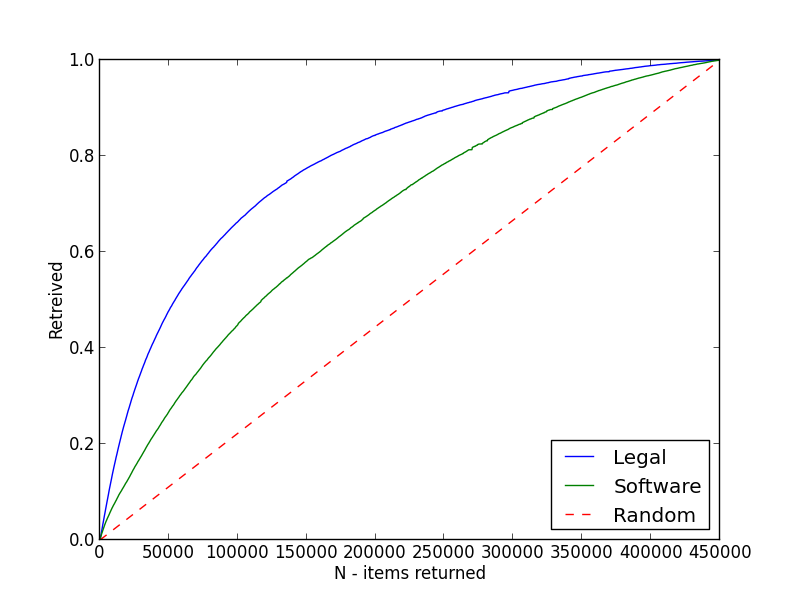
\includegraphics[width=0.5\textwidth]{SVM}
  \caption{Recall graph for the linear SVM over pos-tags.}
  \label{fig:results1}
\end{figure}

\begin{figure}[H]
  \centering
    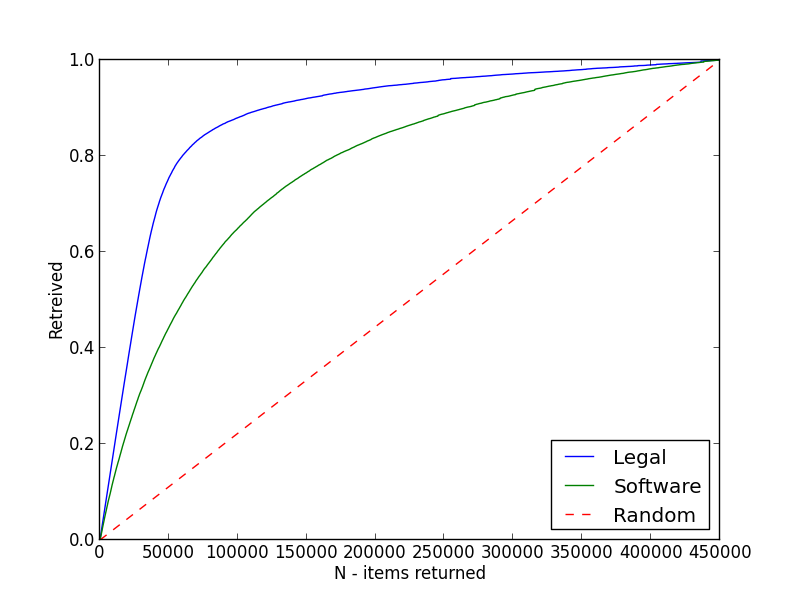
\includegraphics[width=0.5\textwidth]{wbs_0_2}
  \caption{Recall graph for the word-based similarity.}
\label{fig:results2}
\end{figure}

From table \ref{t:t1} and table \ref{t:t2} we can conclude that improving the recall@50.000 will improve the BLEU score. As can be seen in table \ref{t:t2}, the BLEU score improves less in the software domain, where it already starts out higher than in the legal domain. This is consistent with our findings in table \ref{t:t1}, where we find that recall@50.000 is lower in the software domain and conclude that this is because the software domain is already similar to the out-domain corpus. Although using a random method produces higher BLEU in the software domain, applying data selection results in higher BLEU in the legal domain.

\section{Related Work and Discussion}
\label{sec:related}
In domain adaptation one can choose to work on the corpus level (i.e. select data from a general domain corpus that is not relevant to the domain) or on the model level (for example, we could interpolate a general translation model and an in-domain translation model). Smart data selection can be seen as domain adaptation on the corpus level. 

In \cite{pseudo} the authors explore domain adaptation on both the corpus and the model level. To select data from a general domain corpus three simple cross-entropy based models are used: cross-entropy, cross-entropy difference and bilingual cross-entropy. Cross-entropy and cross-entropy difference were both proposed by \cite{intelligent}, who showed that using data selected by using cross-entropy produced better language models that were trained on less data, compared to random data selection. In \cite{pseudo}, it is further concluded that in addition to better language models, using cross-entropy for more intelligent data selection also results in a higher BLEU score in a trained SMT system. In addition to this, the authors also present the performance of cross-entropy difference and bilingual cross-entropy and conclude that selecting data by using bilingual cross-entropy outperforms the other methods. However, although the BLEU scores increase using cross-entropy for data selection, it turns out that the three models are not necessarily good at retrieving the actual in-domain sentences from the general-domain corpus. Instead so-called pseudo in-domain data is extracted from the general domain corpus, which has a different distribution than actual in-domain data. Because of this property, we have decided not to use cross-entropy for data selection, as our approach is focused towards retrieving actual in-domain sentences from a general domain corpus.

Another approach to domain adaptation for SMT is presented in \cite{query} in which the data selection problem is posed as an information retrieval problem. An SMT system is trained using an initial language model. This system is used to translate the test sentences, every possible translation according to the initial system will serve as a hypothesis. Next, the hypotheses are used as queries on the general domain corpus to retrieve sentences that are like the hypothesis (and thus are likely to be similar to the sentences in the in-domain corpus). Using the retrieved sentences the final translation model is trained. The queries can either be bag of words from one or multiple hypotheses, or structured queries where the order of words is preserved. The authors find that the structured query model works best, leading them to the conclusion that preserving word order information while extracting sentences from a general domain corpus improves performance. For future work, we could incorporate the word order in our word-based scoring method. It would be interesting to measure the effect of including the frequency of $n$-ngrams in addition to the frequency of words. Although they have not performed experiments, the authors propose the idea of repeating this process iteratively. Our expansion could also be done iteratively, where we learn a new model for the in-domain sentences based on the training in-domain sentences and the sentences of which it is relatively sure that they are in-domain.

% Misschien beter voor discussie?
%We represent 3 new domain adaptation methods at corpus level. As noted in \cite{pseudo} it is computationally less expensive to filter a corpus than to train multiple translation systems. Our approach is focused towards retrieving the in-domain sentences from a general domain corpus. As found in \cite{pseudo} using cross-entropy methods will not necessarily result in retrieving the in-domain sentences. Therefore, we have devised several new methods that focus on X. As in \cite{query} who use hypotheses to retrieve relevant sentences, we will be exploring methods that will expand the sentences that we have with similar words.

\section{Final remarks}
\label{sec:conclusion}
We have presented two methods for selecting data relevant to a specific domain from a mixed-domain corpus. Training a translation system on mostly in-domain sentences results in significantly higher BLEU scores than when training on a random selection of sentences. The more in-domain sentences that a ranking method can place in the 50.000 sentences that are used to train the translation system, the higher the BLEU score. Pos-tag distribution can be an informative measure to discriminate in and out-domain sentences. For future work we suggest investigating a larger number of domains and yet other methods for sentence ranking, and exploring compression techniques like lemmatisation.  

\begin{thebibliography}{}

\bibitem[\protect\citename{Axelrod \bgroup et al. \egroup} 2011]{pseudo}
Axelrod, Amittai and He, Xiaodong and Gao, Jianfeng
\newblock 2011.
\newblock Domain adaptation via pseudo in-domain data selection.
\newblock Proceedings of the Conference on Empirical Methods in Natural Language Processing, 
355--362
\newblock
Association for Computational Linguistics

\bibitem[\protect\citename{Moore and Lewis}2010]{intelligent}
Moore, Robert C and Lewis, William
\newblock 2010.
\newblock Intelligent selection of language model training data.
\newblock Proceedings of the ACL 2010 Conference Short Papers, 
220--224
\newblock
Association for Computational Linguistics

\bibitem[\protect\citename{Mikolov \bgroup et al.\egroup }2013]{word2vec}
Tomas Mikolov, Kai Chen, Greg Corrado, and Jeffrey Dean.
\newblock 2013.
\newblock Efficient Estimation of Word Representations in Vector Space.
\newblock Proceedings of Workshop at ICLR

\bibitem[\protect\citename{Zhao \bgroup et al. \egroup}2004]{query}
Zhao, Bing and Eck, Matthias and Vogel, Stephan
\newblock 2004.
\newblock Language model adaptation for statistical machine translation with structured query models
\newblock Proceedings of the 20th international conference on Computational Linguistics, 
411
\newblock
Association for Computational Linguistics

%\bibitem[\protect\citename{Mikolov \bgroup et al.\egroup }2013a]{Mikolov:13}
%Tomas Mikolov, Wen-tau Yih, and Geoffrey Zweig.
%\newblock 2013a.
%\newblock Linguistic regularities in continuous space word representations.
%\newblock Proceedings of NAACL-HLT, 
%746--751

%\bibitem[\protect\citename{Mikolov \bgroup et al.\egroup }2013b]{MikolovMT:13}
%Tomas Mikolov, Quoc V. Le and Ilya Sutskever.
%\newblock 2013b.
%\newblock Exploiting Similarities among Languages for Machine Translation.
%\newblock arXiv preprint arXiv:1309.4168, 



\end{thebibliography}

\end{document}
